The vision system also provides a way of tracking the body pose of a person. This is achieved through the
OpenNI open source framework, which provides support for detecting and tracking the body of a human 
in depth images \cite{OpenNI}. OpenNI achieves this by attempting to fit a skeleton on a potential human body. 
The information about the skeleton's joints is used to extract the position and orientation of the body.

The OpenNI module that contains the skeleton fitting capabilities is designed to work exclusively with 
PrimeSense derived sensors \cite{PrimeSensor, NITE}. An example of such sensor is the Microsoft's Kinect 
camera. Similar to the depth-color camera setup described in Chapter \ref{depthcolor}, the Kinect is designed
to capture depth and color images, everything on a single piece of hardware. The Kinect's images can be 
retrieved using the PrimeSense interface provided by OpenNI.

In order to take advantage of OpenNI's body tracking support, the vision system introduces the \KinectCam{} 
class. This class serves both as a representation of the Kinect camera and an interface to the OpenNI 
framework. The \KinectCam{} class is implemented following the same structure as the \ColorCam{} and 
\SwissRangerCam{} classes (see Sections \ref{colorcam} and \ref{swissrangercam}). The \KinectJavaAcquire{}
class establishes the Java interface to OpenNI and as such is used to retrieve the images and body 
skeleton information. The \KinectPacketHandler{} class receives image and skeleton data that is transferred 
over the network. The \KinectReceiver{} uses instances of the two previous classes to handle the data streams 
from the Kinect. A Kinect receiver is used by the \KinectCam{} class to gain access to the image and 
skeleton data. 

This design reveals that, in the \RD{} environment, the Kinect camera is seen not only as a sensor that 
provides depth and color images, but also as a sensor that provides body skeleton data for every image 
frame. The skeleton data is represented with an object of type \KinectSkeleton{}. This object contains the 
position and orientation of every joint in the body skeleton generated by OpenNI. The Kinect receiver handles
the skeleton objects using an instance of the \KinectSkeletonStream{} class, a subtype of \Stream{}. The 
\KinectSkeletonStream{} class represents a sequence of detected body poses, and its design is similar to the 
design of the \FaceStream{} class discussed in Section \ref{facetracker}.

Table \ref{kinectcammethods} lists the methods that the \KinectCam{} class adds to the base camera
representation. The \texttt{get\-Skel\-e\-tons} method further exemplifies the idea that in this system the Kinect
captures image and body skeleton data. The \texttt{cre\-ate\-Dis\-play} method is used to create a color 
visualization of the raw depth data, and the \texttt{thresh\-old} method serves to threshold the values of the
depth image.

\begin{table}[ht]
\caption{Public methods in the \KinectCam{} class}
\begin{center}
\begin{tabular}{| l |}
	\hline 
	\multicolumn{1}{| c |}{\KinectCam{}} \\
	\multicolumn{1}{| c |}{{\small \texttt{extends} \Camera{}}} \\
	\hline \hline
	\texttt{getColor} \\
	\texttt{getDepth} \\
	\texttt{getSkeletons} \\
	\texttt{getDepthDisplay} \\
	\texttt{getColorView} \\
	\texttt{getDepthView} \\
	\texttt{createDisplay} \\
	\texttt{threshold} \\
	\hline
\end{tabular}
\end{center}
\label{kinectcammethods}
\end{table}

Figure \ref{bodyposetrackersequence} shows a sequence of depth images captured with the Kinect camera
along with superimposed red skeletons that illustrate the output of OpenNI's body tracking algorithm. As it has 
been seen before, thresholding the image based on the depth values can segment the body of a person from 
the background assuming there is a significant distance between the two. The top left image shows the position
of the body that is required to calibrate and start the tracking algorithm. The other images show that the 
algorithm is robust to different body positions and orientations. 

One of the principal advantages of the body skeleton data is that it can be used as input to gesture recognition
algorithms. For example, the skeleton can provide information about the position of a person's arms with 
respect to the rest of the body. This information can be used to train algorithms that classify certain arm 
movements into gestures, making possible to recognize, for example, an arm waving, pointing, or reaching out. 

\begin{figure}[t]
\center
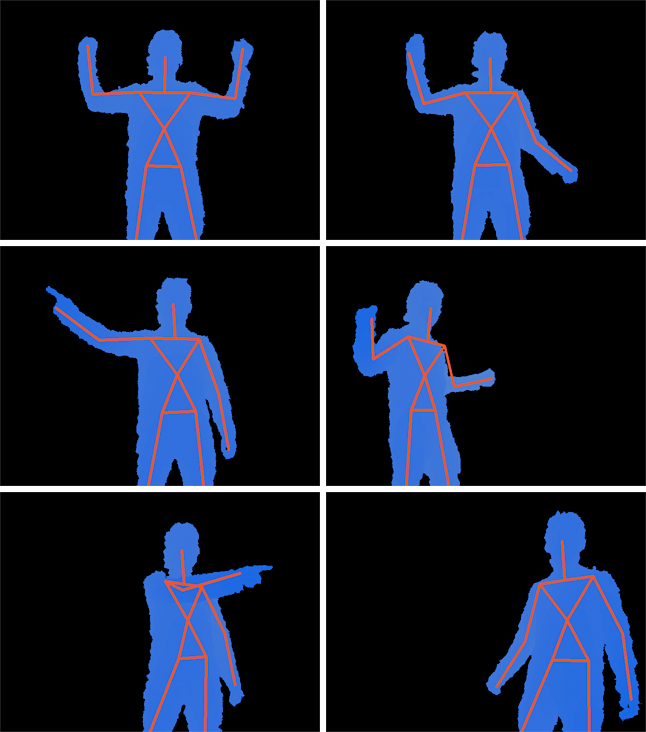
\includegraphics[width = 10cm]{bodyposetracker.png}
\caption[Output of OpenNI's body pose tracking algorithm]{Output of OpenNI's body pose tracking 
algorithm on a sequence of depth images. The red lines indicate the position of the skeleton's joints.}
\label{bodyposetrackersequence}
\end{figure}